% Pdf only
\documentclass[aspectratio=169,12pt]{beamer}
% For presentation
%\documentclass[aspectratio=169, notes]{beamer}

\usepackage{multimedia}
\usepackage{hyperref}

\usepackage{lmodern}
\usepackage{pgfpages}
%\setbeameroption{show notes on second screen}
%\usepackage[utf8]{inputenc} 
\usepackage[english]{babel}

%
% Choose how your presentation looks.
%
% For more themes, color themes and font themes, see:
% http://deic.uab.es/~iblanes/beamer_gallery/index_by_theme.html
%
\mode<presentation>
{
  \usetheme[]{metropolis}           % Use metropolis theme
} 

\setbeamertemplate{note page}{%
  \begin{columns}[c]
    \begin{column}{0.6\linewidth}
      \begin{center}
        \insertslideintonotes{0.5}
      \end{center}
    \end{column}
    \begin{column}{0.4\linewidth}
      \insertnote%
    \end{column}
  \end{columns}
}

\begin{document}
\obeylines

\title[Open Source SLAM Library for Embedded Systems]{Open Source SLAM Library for Embedded Systems}
\author{Stefan Eichenberger, CPVR Lab}
\date{24.01.2020}

\begin{frame}
  \titlepage\thispagestyle{empty}
\end{frame}


\note[itemize]{
  \item Beispiel mit Gleichgewicht
  \item Überleitung zu SLAM
}

\begin{frame}{AR Demo}
  \vspace{-6pt}
  \begin{columns}[T]
    \column{\dimexpr\paperwidth}\centering
    \href{run:ar-demo.mp4?autostart&loop}{\includegraphics[height=0.98\textheight]{out/ar-demo.png}}
  \end{columns}
\end{frame}

\begin{frame}{Different SLAMs}
  \begin{center}
    \includegraphics[height=0.9\textheight]{../img/slam_modes.png}
  \end{center}
\end{frame}

\begin{frame}{Stereo Camera}
  \begin{center}
    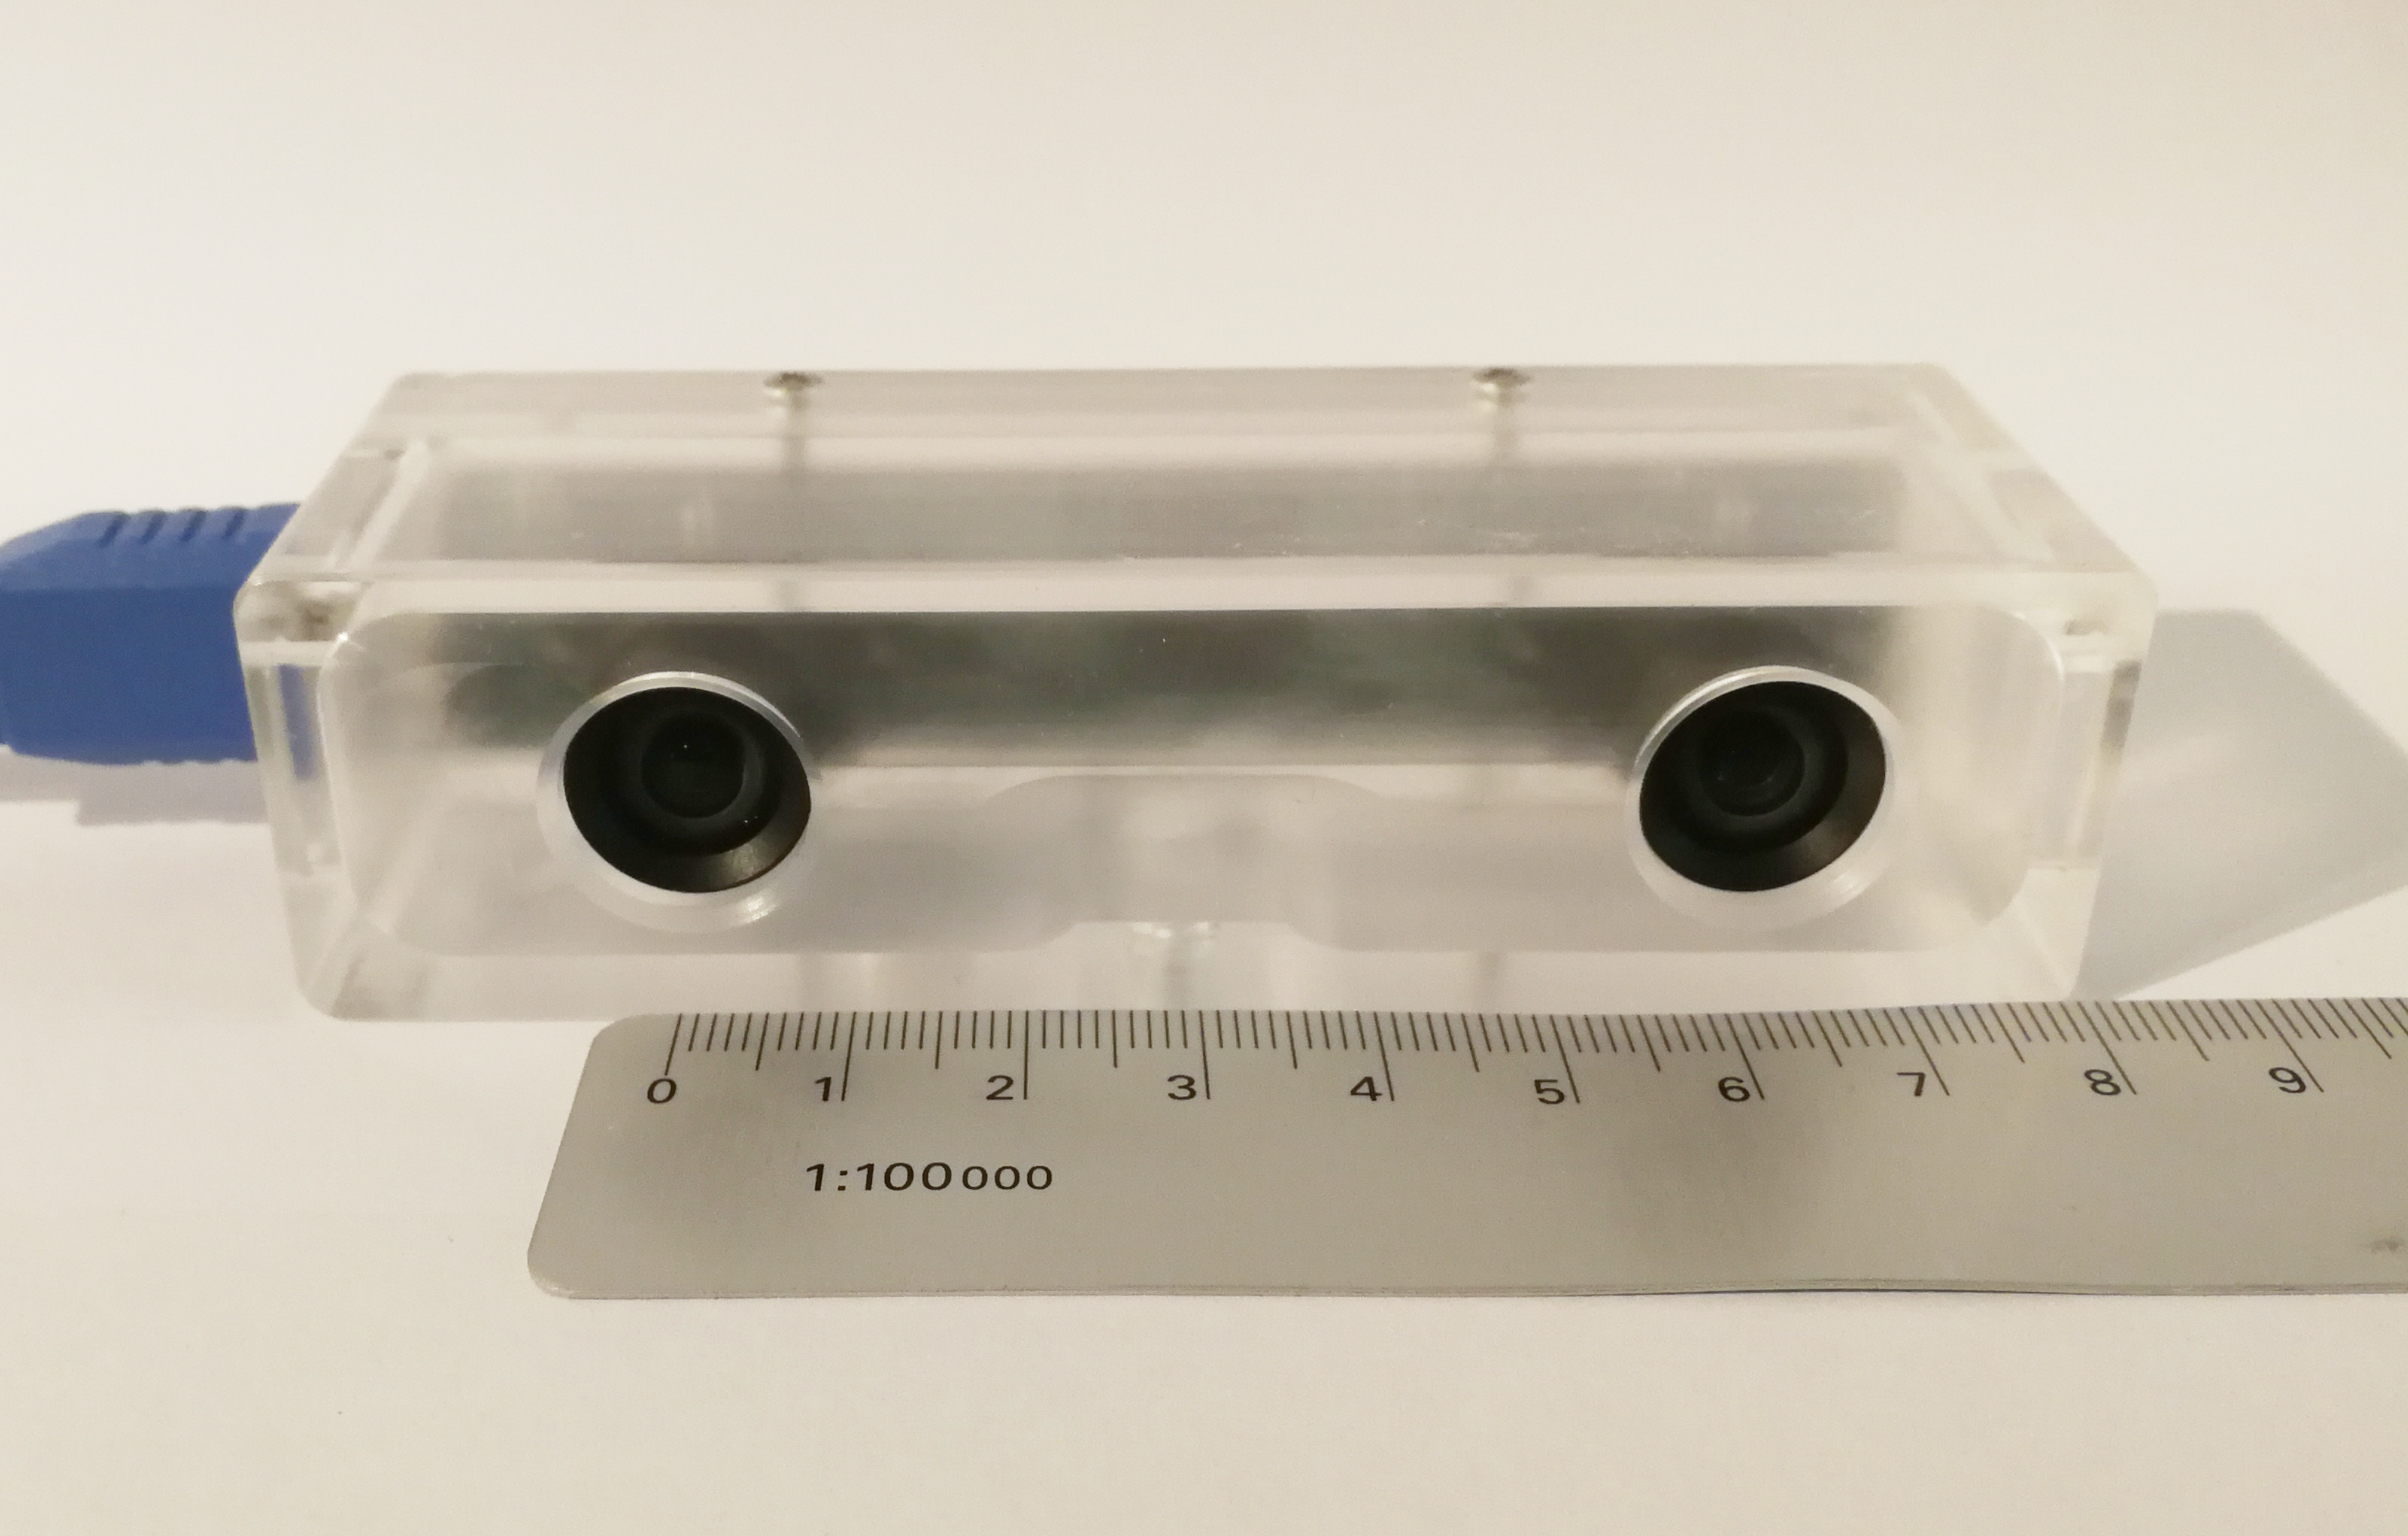
\includegraphics[height=0.9\textheight]{img/tara_cam.png}
  \end{center}
\end{frame}

\note[itemize]{
  \item ECON Tara
  \item Fokus auf Stereo SLAM
}

\begin{frame}{SVO SLAM}
  \begin{center}
    \includegraphics[height=0.95\textheight]{../img/our_svo_slam.png}
  \end{center}
\end{frame}

\begin{frame}{Maintain 3D Point Cloud}
  \begin{columns}[T]
    \begin{column}{0.2\linewidth}
      \begin{tikzpicture}
        \node[anchor=south west,inner sep=0] (image) at (0,0) {\includegraphics[width=1.5\textwidth]{../img/our_svo_slam.png}};
        \begin{scope}[x={(image.south east)},y={(image.north west)}]
            \draw[red,thick] (0.7,0.78) rectangle (0.95,0.45);
        \end{scope}
      \end{tikzpicture}
    \end{column}
    \begin{column}{0.8\linewidth}
      \includegraphics[height=0.95\textheight]{../img/disparity_concept.png}
    \end{column}
  \end{columns}
\end{frame}

\begin{frame}{Sparse Image Alignment}
  \begin{columns}[T]
    \begin{column}{0.2\linewidth}
      \begin{tikzpicture}
        \node[anchor=south west,inner sep=0] (image) at (0,0) {\includegraphics[width=1.5\textwidth]{../img/our_svo_slam.png}};
        \begin{scope}[x={(image.south east)},y={(image.north west)}]
          \draw[red,thick] (0.06,0.59) rectangle (0.52,0.48);
        \end{scope}
      \end{tikzpicture}
    \end{column}
    \begin{column}{0.8\linewidth}
      \includegraphics[height=1.0\textheight]{../img/pose_estimation_sparse.png}
    \end{column}
  \end{columns}
\end{frame}

\begin{frame}{Pose Refinement}
  \begin{columns}[T]
    \begin{column}{0.2\linewidth}
      \begin{tikzpicture}
        \node[anchor=south west,inner sep=0] (image) at (0,0) {\includegraphics[width=1.5\textwidth]{../img/our_svo_slam.png}};
        \begin{scope}[x={(image.south east)},y={(image.north west)}]
          \draw[red,thick] (0.06,0.45) rectangle (0.52,0.34);
        \end{scope}
      \end{tikzpicture}
    \end{column}
    \begin{column}{0.8\linewidth}
      \includegraphics[height=0.9\textheight]{../img/pose_estimation_opt_flow.png}
    \end{column}
  \end{columns}
\end{frame}

\begin{frame}{Pose Refinement}
  \begin{columns}[T]
    \begin{column}{0.2\linewidth}
      \begin{tikzpicture}
        \node[anchor=south west,inner sep=0] (image) at (0,0) {\includegraphics[width=1.5\textwidth]{../img/our_svo_slam.png}};
        \begin{scope}[x={(image.south east)},y={(image.north west)}]
          \draw[red,thick] (0.06,0.45) rectangle (0.52,0.34);
        \end{scope}
      \end{tikzpicture}
    \end{column}
    \begin{column}{0.8\linewidth}
      \includegraphics[height=0.9\textheight]{../img/pose_estimation_refinement.png}
    \end{column}
  \end{columns}
\end{frame}

\begin{frame}{3D Point Update}
  \begin{columns}[T]
    \begin{column}{0.2\linewidth}
      \begin{tikzpicture}
        \node[anchor=south west,inner sep=0] (image) at (0,0) {\includegraphics[width=1.5\textwidth]{../img/our_svo_slam.png}};
        \begin{scope}[x={(image.south east)},y={(image.north west)}]
          \draw[red,thick] (0.06,0.31) rectangle (0.52,0.20);
        \end{scope}
      \end{tikzpicture}
    \end{column}
    \begin{column}{0.8\linewidth}
      \includegraphics[height=0.9\textheight]{../img/pose_estimation_point_update.png}
    \end{column}
  \end{columns}
\end{frame}

\begin{frame}{Optical Flow}
  \begin{columns}[c]
    \column{\dimexpr\paperwidth}
    \begin{center}
      \includegraphics[width=0.95\textwidth]{img/optical_flow_intuitive_1.png}
    \end{center}
  \end{columns}
\end{frame}

\begin{frame}{Optical Flow}
  \begin{columns}[c]
    \column{\dimexpr\paperwidth}
    \begin{center}
      \includegraphics[width=0.95\textwidth]{img/optical_flow_intuitive_2.png}
    \end{center}
  \end{columns}
\end{frame}

\begin{frame}{Optical Flow}
  \begin{columns}[c]
    \column{\dimexpr\paperwidth}
    \begin{center}
      \includegraphics[width=0.6\textwidth]{img/optical_flow_intuitive_3.png}
    \end{center}
  \end{columns}
\end{frame}

\begin{frame}{Optical Flow}
  \begin{columns}[c]
    \column{\dimexpr\paperwidth}
    \begin{center}
      \includegraphics[width=0.95\textwidth]{../img/optical_flow_2d.png}
    \end{center}
  \end{columns}
\end{frame}

\begin{frame}{Results (Blender Scene)}
  \vspace{-6pt}
  \begin{columns}[T]
    \column{\dimexpr\paperwidth}\centering
    \href{run:blender-classroom.mkv?autostart&loop}{\includegraphics[height=0.98\textheight]{out/blender-classroom.png}}
  \end{columns}
\end{frame}

\begin{frame}{Results}
  \begin{columns}[c]
    \column{\dimexpr\paperwidth}
    \begin{center}
      \includegraphics[height=0.9\textheight]{img/blender_classroom_simple_comp_top.png}
    \end{center}
  \end{columns}
\end{frame}

\begin{frame}{Conclusion}
  \begin{columns}[c]
    \begin{column}{0.4\linewidth}
      \begin{itemize}
        \item Faster than ORB SLAM
        \item Not as accurate
        \item Good for embedded devices
        \item Less beneficial for CPVR lab
      \end{itemize}
    \end{column}
    \begin{column}{0.4\linewidth}
      \begin{center}
        \includegraphics[width=0.5\textwidth]{./img/exclamationmark.jpg}
      \end{center}
    \end{column}
  \end{columns}
\end{frame}

\begin{frame}{Questions}
  \begin{center}
    \includegraphics[height=0.7\textheight]{./img/question.jpg}
    https://github.com/eichenberger/stereo-svo-slam
  \end{center}
\end{frame}


\end{document}

